\newcommand{\electronic}[2]{#2} % #1 = printer friendly version, #2 = screen viewing version

\electronic{\documentclass[article]{memoir}}{\documentclass[article,openany]{memoir}}

\usepackage{amsmath,amssymb, amsthm}
\usepackage[usenames,dvipsnames]{xcolor}
\definecolor{darkgreen}{rgb}{0,0.5,0}
\definecolor{darkblue}{rgb}{0,0,0.5}

\usepackage[latin1]{inputenc}
\usepackage[T1]{fontenc}
\usepackage{lmodern}
\usepackage{graphicx}
\usepackage{caption}
\usepackage{subcaption}
\usepackage[pdftex,bookmarks,raiselinks,pageanchor,hyperindex,colorlinks,\electronic{urlcolor=black,linkcolor=black,citecolor=black}{urlcolor=darkblue,linkcolor=darkblue,citecolor=darkgreen}]{hyperref}
\usepackage{lstdoc}
\usepackage{longtable}

\electronic{\setlrmarginsandblock{*}{4.0cm}{0.75}}{\setlrmarginsandblock{*}{3.5cm}{1}}
\setulmarginsandblock{3.0cm}{*}{1.2}
\checkandfixthelayout

\renewcommand{\bibname}{References}

\urlstyle{sf}

\newcommand{\relmiddle}[1]{\mathrel{}\middle#1\mathrel{}}

\newcommand{\abs}[1]{\lvert #1 \rvert}
\newcommand{\Abs}[1]{\lVert #1 \rVert}
\newcommand{\dd}{\partial}

\newcommand{\id}{\mathrm{id}}
\newcommand{\Int}{\operatorname{Int}}

\renewcommand{\bar}{\overline}

\newcommand{\bbR}{\mathbb{R}}
\newcommand{\bbC}{\mathbb{C}}
\newcommand{\bbN}{\mathbb{N}}
\newcommand{\bbQ}{\mathbb{Q}}
\newcommand{\bbZ}{\mathbb{Z}}

\newcommand{\calB}{\mathcal{B}}
\newcommand{\calC}{\mathcal{C}}
\newcommand{\calP}{\mathcal{P}}
\newcommand{\calT}{\mathcal{T}}

\newcommand{\eps}{\varepsilon}
\renewcommand{\epsilon}{\varepsilon}
\renewcommand{\phi}{\varphi}


\theoremstyle{plain}
\newtheorem{lem}{Lemma}[section]
\newtheorem{thm}[lem]{Theorem}
\newtheorem{prop}[lem]{Proposition}
\newtheorem{cor}[lem]{Corollary}
\newtheorem{badjoke}[lem]{Bad joke}

\theoremstyle{definition}
\newtheorem{defn}[lem]{Definition}
\newtheorem{example}[lem]{Example}

\theoremstyle{remark}
\newtheorem{rem}[lem]{Remark}

\makechapterstyle{combined}{
  \setlength{\midchapskip}{10pt}
  \setlength{\afterchapskip}{2.5cm}
  \renewcommand*{\printchaptername}{}
  \renewcommand*{\chapnumfont}{\normalfont\sffamily\bfseries\fontsize{42}{0}\selectfont}
  \renewcommand*{\printchapternum}{\flushright\normalfont\sffamily\Huge\bfseries Chapter \chapnumfont{\thechapter}}
  \renewcommand*{\chaptitlefont}{\normalfont\sffamily\bfseries\Huge}
  \renewcommand*{\printchaptertitle}[1]{\bfseries\chaptitlefont{##1}}
    %\raggedright\chaptitlefont\parbox[t]{\textwidth}{\raggedright##1}}
}
\chapterstyle{combined}

\renewcommand{\secheadstyle}{\sffamily\LARGE\bfseries}
\renewcommand{\subsecheadstyle}{\sffamily\Large\bfseries}
\counterwithout{section}{chapter}
\setsecnumdepth{subsection}
\setcounter{tocdepth}{2}

\makeindex

%%%%% End preample

\begin{document}

% Commands related to the index and the list of translations.
% This one is largely taken from
%   https://tex.stackexchange.com/questions/19746/cunning-latex-tricks/19761#19761

\makeatletter
\let\alist\@empty
\newcommand{\addtolist}[2]{\lst@lAddTo#1{#2}}
\newcommand{\trans}[2]{\addtolist{\alist}{#1#2,}\expandafter\gdef\csname#1#2\endcsname{#1&#2\cr\relax}\lst@BubbleSort{\alist}}
\newcommand{\wordexp}[4]{\emph{#1} (sv: \emph{#2})\index{#3}\addtolist{\alist}{#3#4,}\expandafter\gdef\csname#3#4\endcsname{#3&#4\cr\relax}\lst@BubbleSort{\alist}}
\newcommand{\word}[2]{\wordexp{#1}{#2}{#1}{#2}}

\frontmatter
\pretitle{\begin{center}\Huge\bfseries}
\title{Basic topology}
\posttitle{
  \par\vskip1em{\normalfont\normalsize\scshape Lecture notes for a 2015 Uppsala University course\par\vfill}
  \includegraphics[width=\textwidth]{images/stereo-frontpage}
  \end{center}
}
\author{S{\o}ren Fuglede J{\o}rgensen}
\predate{\vfill\begin{center}\large Version: }

\begin{titlingpage}
\maketitle
\end{titlingpage}

\tableofcontents
\section{Preface}
\label{preface}
These are lecture notes written for a course on elementary point set topology given at Uppsala University during the spring of 2015. The notes are, at the time of writing, \emph{not} intended as a full reference for the course. Rather, the course will follow the references \cite{Mun} and \cite{Fje}, and these notes serve to show which parts of the main references we have covered in the lectures.

The notes will be written as the course moves along and may be discontinued at any moment, depending on time restrictions. As such, they are also likely to contain typos and errors of other kinds; if you come across any such, feel very free to let me know, either by email at \href{mailto:s@fuglede.dk}{\textsf{s@fuglede.dk}}, or by letting me know in person. Concrete changes can also be proposed directly at \href{https://github.com/fuglede/basic-topology}{\textsf{https://github.com/fuglede/basic-topology}}.

\section{Introduction}
\label{introduction}
This course will mainly be concered with the study of topological spaces. Topological spaces are abstract mathematical concepts whose definition include a sufficient amount of data for them to be called ``spaces''. Familiar spaces would be something like $\mathbb{R}^3$ or $\mathbb{R}^n$, but more abstract objects -- such as general vector spaces -- we also think of as ``spaces''. On the other hand, in algebra one encounters objects such as groups and rings that one would generally not think of as spaces, and on the extreme side we talk about sets, which are more general ``collections of things'' which we may or may not choose to think of as spaces.

From this point of view, one might think of topological spaces with an added bit of \word{structure}{struktur}\footnote{See \url{https://en.wikipedia.org/wiki/Mathematical_structure} for a more precise discussion.}; a term used throughout mathematics but typically with a rather vague meaning. As such, sets have no interesting structure, but Euclidian space $\mathbb{R}^n$ has plenty: for instance, the usual inner product $\langle \cdot ,\cdot \rangle$ on $\mathbb{R}^n$ can be used to talk about angles between vectors. This in turn can be used to define the standard norm $\lVert \cdot \rVert$ on $\mathbb{R}^n$ which allows us to talk about lengths of vectors and distances between points. All of this is structure that may not be given to us in a general vector space, but without having this structure on $\mathbb{R}^n$, there would be no such thing as calculus: we wouldn't be able to define things like differentiability and continuity.

For topological spaces we discard all of this fine structure, so that in particular it makes no sense to talk about the distance between two points in a general topological space. The only piece of structure that we will require is that of ``open sets'': given a subset of a topological space, we want to be able to tell if it is open or not. This turns out to be the least amount of structure needed to define continuity, so the study of topological spaces is very much the study of continuous functions.

The study of general topological spaces and continuous functions will be contained in Sections~\ref{topological-spaces}--\ref{homeomorphisms}. Simply having open sets turns out also to be sufficient to talk about what it means for a space to be ``connected'' and ``compact'' in a way that corresponds to what one would normally associate with those words. More abstractly, we will also look at the notion of separating points, which is less familiar in examples like $\mathbb{R}^n$. These properties of topological spaces will be the basis of Sections~\ref{connectedness}--\ref{separation}.

The study of general topological spaces and their fundamental properties is often referred to as \word{point-set topology}{punktm{\"a}ngdstopologi} or \word{general topology}{allm{\"a}n topologi}. The less structure a certain space has, the less deep the mathematical results about it tends to be, and out treatment will involve correspondly few deep mathematical theorems; rather, for the first part of the course, one should think of the materials as developing the necessary tools to deal with topological spaces in other contexts. Towards the end of the course, we will remedy this by tying together our theory with other parts of mathematics. Concretely, in Section~\ref{homotopy} we touch upon the mathematical area of \word{algebraic topology}{algebraisk topologi} which is concerned with analyzing certain natural algebraic structures that can be associated with topological spaces, and in Section~\ref{manifolds}, we will study a particular nice family of topological spaces called manifolds that show up in all of geometry.

Before being able to do any of this, though, we need to firmly settle on what sets are, and how one deals with them.


\mainmatter
\section{Set theory and logic}
\label{set-theory}
Here's a \word{set}{m{\"a}ngd} with a \word{topology}{topologi}.

\section{Topological spaces}
\label{topological-spaces}

\section{Homeomorphisms and distinguishability}
\label{homeomorphisms}
Often in mathematics, when talking about objects as certains things coming with certain structures, we want to be able to say when two objects are ``the same''. Consider for instance the two topological spaces $X = \{ 1 , 2 , 3 \}$ and $Y = \{ 4, 5, 6 \}$ with the topologies
\begin{align*}
  \calT_X &= \{ \emptyset, \{1 \}, \{ 2 \}, \{ 1, 2 \}, \{1,2,3\} \}, \\
  \calT_Y &= \{ \emptyset, \{4 \}, \{ 5 \}, \{ 4, 5 \}, \{4,5,6\} \}.
\end{align*}
These spaces are not particularly different for if we identify $1 \leftrightarrow 4$, $2 \leftrightarrow 5$, $3 \leftrightarrow 6$, we have no way to tell them apart. This notion of being the same is made precise in the definition of a ``homeomorphism'' below.

The well-educated mathematics student will have likely come across this general idea before: we consider two vector spaces the same if there is a linear isomorphism from one to the other, we consider algebraic objects such as groups and rings the same if they are isomorphic, and if all we know about two given sets is that they are in bijection, we may as well treat them as the same. This language of ``objects'' being ``the same'' is unified in the branch of mathematics called \word{category theory}{kategoriteori}, sometimes referred to as \emph{abstract nonsense}\index{abstract nonsense}. We will be discussing category theory in any detail in these notes, but it is useful to be aware of its existence.

\subsection{Homeomorphisms}
In the example above, we notice that crucial property of two topological spaces that ``are the same'' is that they are in bijection and have the same open sets. This leads to the following definition.
\begin{defn}
  A bijection $f : X \to Y$ between two topological spaces is called a \word{homeomorphism}{homeomorfi} if $f$ and its inverse $f^{-1}$ are continuous. In this case, we say that $X$ and $Y$ are \word{homeomorphic}{homeomorfa} and we write $X \simeq Y$.
\end{defn}
Equivalently, since a bijection $f$ always satisfies $f = (f^{-1})^{-1}$, one could define a homeomorphism to be a bijection such that $f(U)$ is open whenever $U$ is. Notice also that $\simeq$ satisfies the property of an equivalence relation.
\trans{homeomorphism}{homeomorfi}\trans{homeomorphic}{homeomorfa}
\begin{example}
  In the example in the beginning of this section, the bijection $f : X \to Y$ given by $f(1) = 4$, $f(2) = 5$, $f(3) = 6$ is a homeomorphism.
\end{example}
\begin{example}
  Let $f : (-1 , 1) \to \bbR$ be the bijective map
  \[
    f(x) = \tan \left( \frac{\pi x}{2} \right)
  \]
  whose inverse is $f^{-1}(x) = \tfrac{2}{\pi} \arctan x$. Then both $f$ and $f^{-1}$ are continuous so $(-1,1)$ and $\bbR$ are isomorphic.
\end{example}
From the above example we conclude that two spaces that we are otherwise familiar with and think of as different may turn out to be the same from the viewpoint of topology. Roughly, since we don't care about the scale of $(-1,1)$ but only its open sets, we are able to stretch it as much as we please, and end up with something like $\bbR$
\begin{badjoke}
  Let $A$ be a typical topologist. Then $A$ is not able to tell the difference between her coffee mug and her donut.
\end{badjoke}
\begin{proof}
  The surfaces of the coffee mug and the donut are homeomorphic. See \url{https://upload.wikimedia.org/wikipedia/commons/2/26/Mug_and_Torus_morph.gif}.
\end{proof}
\begin{example}
  Let $B^n := B(0,1)$ be the unit ball in $\bbR^n$. Then $B^n \simeq \bbR^n$. This can be seen because the map $f : B^n \to \bbR^n$ given by
  \[
    f(x) = \frac{x}{1-\Abs{x}}
  \]
  is a continuous bijection with inverse
  \[
    f^{-1}(x) = \frac{x}{1+\Abs{x}}.
  \]
\end{example}
We will often be interested in functions that would be homeomorphisms if we were allowed to shrink the codomain appropriately.
\begin{defn}
  Let $X$ and $Y$ be topological spaces. A function $f: X \to Y$ is called an \word{embedding}{?} if $f : X \to f(X)$ is a homeomorphism; here $f(X)$ has the subspace topology from $Y$.
\end{defn}
\begin{example}
  If $X$ is a topological space and $Y \subset X$ a subspace, then the inclusion $\iota : Y \to X$ given by $\iota(x) = x$ is an embedding.
\end{example}

\subsection{Topological invariants}
Above, we have talked about what it means for two topological spaces to be the same. Often, one will be interested in the converse question of telling two topological spaces apart. As such, we consider topological spaces different if they are non-homeomorphic; for instance, if $X = \{a,b\}$ then we obtain two different topological spaces by equipping it with the trivial and the discrete topology.

\begin{defn}
  Let \textbf{Top} denote the collection of \emph{all} topological spaces. A \emph{topological invariant}, sometimes called a \emph{topological property}, is a function $f$ defined on \textbf{Top} so that if $X \simeq Y$, then $f(X) = f(Y)$.
\end{defn}
The important thing to note is that if $f$ is a topological invariant and $f(X) \not= f(Y)$, then $X$ and $Y$ are not homeomorphic. Thus we are lucky enough, we can use topological invariants to tell topological spaces apart.
\begin{example}
  Let $f : \textbf{Top} \to \{ \text{yes}, \text{no} \}$ be the function given by answering the question ``is $X$ Hausdorff?'' That is
  \[
    f(X) = \begin{cases} \text{yes}, &\text{ if $X$ is Hausdorff,}\\ \text{no}, &\text{ if $X$ is not Hausdorff.} \end{cases}
  \]
  Then $f$ is a topological invariant: if $X \simeq Y$ and $X$ is Hausdorff, then so is $Y$. For this reason, the property of being Hausdorff is often called a topological property. Again, one can turn this around and say that if $X$ is Hausdorff but $Y$ is not, then $X$ and $Y$ are not homeomorphic. Similarly, being $T_0$ or $T_1$ are topological properties. As is being first-countable and any other property that is defined using only in terms of open sets.
\end{example}

We will encounter many other topological properties later on, one of the most important ones being the fundamental group, which is to be introduced in Section~\ref{homotopy}.

\subsection{The $n$-dimensional sphere}
\begin{defn}
  The \emph{$n$-sphere} is the set
  \[
    S^n = \{ x \in \bbR^{n+1} \mid \Abs{x} = 1 \} \subset \bbR^{n+1}
  \]
  with the subspace topology from $\bbR^{n+1}$.
\end{defn}
\begin{prop}
  Let $p = (0,0,\dots,0,1) \in S^n$ be the ``north pole''. Then $S^n \setminus \{p\} \simeq \bbR^n$.
\end{prop}
\begin{proof}
  We will construct a homeomorphism explicitly, leaving some of the details to the reader. Let $x = (x_1, \dots, x_{n+1}) \in S^n \setminus \{ p \}$ so that $x_{n+1} \not= 1$. We then define the \word{stereographic projection}{stereografisk projektion} of $x$ by
  \[
    \Pi(x) = \Pi(x_1,\dots,x_n,x_{n+1}) = \frac{1}{1-x_{n+1}) (x_1, \dots, x_n) \in \bbR^n.
  \]
  Geometrically, if one draws a straight line through $x$ and $p$, then its intersection with $\bbR^n \times \{0 \}$ will be the point $(\Pi(x),0)$. Now $\Pi$ is continuous because each of its components are (use Proposition~\ref{props-subspace-top}), and one can check that it has an inverse $g : \bbR^n \to S^n \setminus \{p \}$ given by
  \[
    g(y_1, \dots, y_n) = (t(y) y_1, \dots, t(y)y_n, 1-t(y)),
  \]
  where $t(y) = 2/(1+\Abs{y}^2)$.
\end{proof}
\begin{remark}
  If $q = (0,\dots,0,-1) \in S^n$ is the south pole, then the map $(x_1, \dots, x_n,x_{n+1}) \mapsto (x_1,\dots,x_n,-x_{n+1})$ is a homeomorphism from $S^n \setminus \{p\}$ to $S^n \setminus \{ q \}$, so we also have that $S^n \setminus \{ q \}$ is homeomorphic with $\bbR^n$. More generally, one can show $S^n \setminus \{x\} \simeq \bbR^n$ for all $x \in S^n$.
\end{remark}
\begin{example}
  Let $f : [0,1) \to S^1$ be the map $f(x) = (\cos (2\pi x), \sin(2\pi x))$. Then $f$ is a bijection with inverse $f^{-1}(x,y) = \arcsin(y)/(2\pi)$. Moreover, $f$ is continuous: Let $U \subset S^1$ be open. Then there is an open set $V$ in $\bbR^2$ so that $U = S^1 \cap V$.
\end{example}

\section{Connectedness}
\label{connectedness}
In $\bbR^n$, we have a good intuituion about what it means for subsets to be connected or not. For example, the subset $(-2,-1) \cup (1,2)$ does seem very connected: how would we connect $-1$ and $1$? On the other hand, $(-2,2)$ should probably deserve to be called connected.

It turns out that having open sets is sufficient to define a notion of connectedness that agrees with out intuition in the intuitive examples; this is the subject of this sections.

\subsection{Connectedness}
\begin{defn}
  Let $X$ be a topological space. A \word{separation}{?} of $X$ is a pair $U$, $V$ of disjoint non-empty open subsets of $X$ so that $X = U \cup V$. We say that $X$ is \word{connected}{sammanh{\"a}ngande} if it has no separation.
\end{defn}
\trans{separation}{?}\trans{connected}{sammanh{\"a}ngande}
In the following we will often be dealing with connectedness of subspaces. Keep in mind that when doing so, the subspace will always be equipped with the subspace topology.
\begin{example}
  The subspace $(-2,-1) \cup (1,2) \subset \bbR$ has a separation.
\end{example}
Notice that if $X = U \cup V$ is a separation, then $U = X \setminus V$ and $V = X \setminus U$. This means that both $U$ and $V$ are both open and closed.
\begin{lem}
  A topological space $X$ is connected if and only if $\emptyset$ and $X$ are the only subsets of $X$ that are both open and closed.
\end{lem}
\begin{proof}
  Suppose that $U \subset X$ is both open and closed. Then $V = X \setminus U$ is open, and $X = U \cup V$ is a separation. If $X$ is connected one of $U$ and $V$ must be empty, since otherwise we would have a separation of $X$.
\end{proof}
% \begin{lem}
%   A topological space $X$ is connected if and only if the following condition holds: if $X = C \cup D$ where $C$ and $D$ are disjoint closed subsets of $X$, then either $C = \emptyset$ or $D = \emptyset$.
% \end{lem}
% \begin{proof}
%   Exercise.
% \end{proof}
\begin{example}
  The rational numbers $\bbQ \subset \bbR$ are not connected: choose any irrational number $a \in \bbR$. Then
  \[
    \bbQ = ((-\infty, a) \cup (a,\infty)) \cap \bbQ = ((-\infty,a) \cap \bbQ) \cup (\bbQ \cap (a,\infty)),
  \]
  which is a separation by definition of the subspace topology on $\bbQ$.
\end{example}
\begin{example}
  \label{discrete-connectedness}
  If $X$ has the discrete topology and consists of more than two points, then $X = \{x\} \cup (X \setminus \{x\})$ is a separation of $X$, so $X$ is not connected.
\end{example}
\begin{example}
  Intervals in $\bbR$ are connected. This looks extremely reasonable from the intuition about connectedness provided above, but we will only show it as a consequence of a few general results that we now turn to.
\end{example}
\begin{lem}
  \label{connectedness-subspace-lemma}
  Let $X = U \cup V$ for disjoint open sets $U$ and $V$, and let $Y \subset X$ be a subspace. If $Y$ is connected, then $Y \subset U$ or $Y \subset V$.
\end{lem}
\begin{proof}
  We will show the contrapositive of the statement, so assume that $Y \cap U \not= \emptyset$ and $Y \cap V \not= \emptyset$. Then
  \[
    Y = Y \cap X = Y \cap (U \cup V) = (Y \cap U) \cup (Y \cap V)
  \]
  is a separation of $Y$, since $Y \cap U$ and $Y \cap V$ are disjoint, non-empty and open in the subspace topology. Thus $Y$ is not connected.
\end{proof}
\begin{thm}
  Let $\{A_i\}_{i \in I}$ be a collection of connected subspaces of a topological space $X$ with a common point $x \in X$; i.e. $x \in A_i$ for all $i \in I$. Then $\bigcup_{i \in I} A_i$ is connected.
\end{thm}
\begin{proof}
  Suppose that $\bigcup_{i \in I} A_i = U \cup V$ for disjoint subsets $U$ and $V$ that are open in $\bigcup_{i \in I} A_i$ and let us show that either $U$ or $V$ must be empty. Assume without loss of generality that $x \in U$. By Lemma~\ref{connectedness-subspace-lemma} we have for each $i$ that either $A_i \subset U$ or $A_i \subset V$. Since $x \in A_i$ we must have $A_i \subset U$ for all $i \in I$. This implies that $\bigcup_{i \in I} A_i \subset U$, so $V$ must be empty.
\end{proof}
\begin{thm}
  Let $A \subset X$ be connected. If a subset $B \subset X$ satisfies $A \subset B \subset \bar A$, then $B$ is also connected. In particular, $\bar A$ is connected when $A$ is.
\end{thm}
\begin{proof}
  Suppose that $B = U \cap V$ for disjoint subsets $U$ and $V$ that are open in $B$. Then by Lemma~\ref{connectedness-subspace-lemma} we must have that $A \subset U$ or $A \subset V$, so assume without loss of generality that $A \subset U$. Then $B \subset \bar A \subset \bar U$ (where all closures are in the bigger space $X$).
  
  By definition of the subspace topology, there are open sets $U'$ and $V'$ in $X$ so that $U = B \cap U'$, $V = B \cap V'$, and
  \[
    U = B \setminus V = B \setminus (B \cap V') \subset X \setminus V'.
  \]
  The latter space is closed so $\bar U \subset X \setminus V' \subset X \setminus V$. Putting this together, $B \subset X \setminus V$ which means that $B \cap V = \emptyset$, so $V = \emptyset$, and so $B$ is connected.
\end{proof}
\begin{thm}
  \label{images-of-connected}
  Let $f : X \to Y$ be a continuous map between two topological spaces. If $X$ is connected, then $f(X)$ is also connected.
\end{thm}
\begin{proof}
  Suppose that $f(X) = U \cup V$ for disjoint subsets $U$ and $V$ that are open in $f(X)$. Then $f^{-1}(U)$ and $f^{-1}(V)$ are disjoint open subsets of $X$ with $X = f^{-1}(U) \cup f^{-1}(V)$. This means that either $f^{-1}(U)$ or $f^{-1}(V)$ is empty. Suppose that $f^{-1}(U)$ is empty. Then since $U \subset f(X)$ we must have $U = \emptyset$.
\end{proof}
\begin{cor}
  Let $X$ be a connected topological space, and let $Y$ be any set. Suppose that $f : X \to Y$ is a locally constant map, meaning that every point $x \in X$ has a neighbourhood $U$ so that $f|_U$ is constant. Then $f$ is constant.
\end{cor}
\begin{proof}
  Give $Y$ the discrete topology. Then the condition that $f$ is locally constant implies that $f$ is continuous at every point, so $f$ is continuous. Thus $f(X)$ is connected by Theorem~\ref{images-of-connected}, but $f(X)$ also has the discrete topology, so by Example~\ref{discrete-connectedness} it consists of a single point which is the same as saying that $f$ is constant.
\end{proof}
\begin{thm}
  If $\{X_i\}_{i \in I}$ is a family of topological spaces, then their product $\bigprod_{i \in I} X_i$ is connected if and only if every $X_i$ is.
\end{thm}
\begin{proof}
  Suppose that the product is connected. Recall that the projection $\pi_j : \bigprod_{i \in I} X_i \to X_j$ is continuous for every $j$, so every $X_j$ is connected by Theorem~\ref{images-of-connected}.
  
  Let us show the converse in the case where $I$ is finite. The infinite case is left as an Exercise.
\end{proof}

\section{Compactness and sequential compactness}
\label{compactness}
\section{compactness}
\begin{defn}
  Let $(X,\calT)$ be a topological space.
  \begin{itemize}
    \item[(i)] A collection $\calU \subset \calT$ of open sets of called an \word{open cover}{{\"o}ppen {\"o}vert{\"a}ckning} of $X$ if $X = \bigcup_{U \in \calU} U$.
    \item[(ii)] The space $X$ is called \word{compact}{kompakt} if \emph{every} open cover $\calU$ of $X$ has a finite subcover, meaning that one can find finitely many open sets $U_1, \dots, U_n \in \calU$ so that $X = \bigcup_{i=1}^n U_i$.
  \end{itemize}
\end{defn}
\trans{open cover}{{\"o}ppen {\"o}vert{\"a}ckning}
\trans{compact}{kompakt}

\section{Separation and countability axioms}
\label{separation}
We encountered the first separation axioms in Section~\ref{separation-1}; in this section we introduce further notions of separations. We have already seen how the property of being $T_2$ allows many useful results, and in the same spirit we will see how having more fine-grained separation allows for further characterisation of topological spaces.
\subsection{Separation -- part 2}
\begin{defn}
  A topological space is called \word{regular}{regulj{\"a}rt} if for every closed set $F \subset X$ and any point $x \in X \setminus F$ there exist open sets $U_x, U_F \subset X$ so that $x \in U_x$, $F \subset U_F$, and $U_x \cap U_F = \emptyset$.
  
  A regular $T_1$-space is called $T_3$\index{T_3}.
\end{defn}
\trans{regular}{regulj{\"a}rt}

\section{Introduction to homotopy theory}
\label{homotopy}
In this final section of this note, we will introduce a powerful topological invariant. In doing so, we tread slightly into the realm of algebraic topology.

\subsection{Homotopy}
\begin{defn}
  Let $X$ and $Y$ be topological spaces, and let $f, g : X \to Y$ be continuous maps. We say that $f$ is \word{homotopic}{homotop} to $g$ if there exists a continuous map $F : X \times [0,1] \to Y$ so that
  \[
    F(x,0) = f(x) \quad \text{and} \quad F(x,1) = g(x)
  \]
  for all $x \in X$. The map $F$ is called a \word{homotopy}{homotopi} from $f$ to $g$, and we write $f \sim g$. If $f \sim g$ where $g$ is a constant map, we say that $f$ is \word{null-homotopic}{nollhomotop}
\end{defn}
\trans{homotopic}{homotop}
\trans{homotopy}{homotopi}
\trans{null-homotopic}{nollhomotop}
We will primarily be interested in the special case where the maps $f$ and $g$ are paths that start and end at the same point. In this case, we will furthermore require that the homotopy fixes the two end-points of the paths:
\begin{defn}
  Two $\gamma, \gamma' : [0,1] \to X$ be two paths from $x$ to $y$ in a topological space $X$. We say that $\gamma$ is \word{path homotopic}{v{\"a}ghomotop} to $\gamma'$ if there is a homotopy $F: [0,1] \times [0,1] \to X$ from $\gamma$ to $\gamma'$ so that
  \[
    F(0,t) = x, \quad F(1,t) = y
  \]
  for all $t \in [0,1]$. The map $F$ is called a \word{path homotopy}{v{\"a}ghomotopi}, and we write $\gamma \sim_p \gamma'$. See Figure~\ref{path-homotopy-figure}.
\end{defn}
\begin{figure}
  \centering
  \begin{overpic}{images/path-homotopy}
    \put(33,34){$\gamma$}
    \put(57,46){$\gamma'$}
  \end{overpic}
  \caption{Two homotopic paths $\gamma$ and $\gamma'$ in $\bbR^2$ as well as a path homotopy $F$ between them. That is, we picture $F(s,0) = \gamma(s)$, $F(s,1) = \gamma'(s)$, the paths $F(s,\tfrac{1}{10}), F(s,\tfrac{2}{10}), \dots, F(s,\tfrac{9}{10})$ (in red) and the paths $F(\tfrac{1}{10},t), F(\tfrac{2}{10},t), \dots, F(\tfrac{9}{10},t)$ (in blue).}
  \label{path-homotopy-figure}
\end{figure}
\trans{path homotopic}{v{\"a}ghomotop}
\trans{path homotopy}{v{\"a}ghomotopi}
\begin{lem}
  Homotopy $\sim$ and path homotopy $\sim_p$ are equivalence relations.
\end{lem}
\begin{proof}
  Let $f, g, h : X \to Y$ be continuous maps.
  
  To see reflexivity, define $F : X \times [0,1] \to Y$ by $F(x,t) = f(x)$. Then $F$ is continuous and $F(x,1) = F(x,0) = f(x)$ for all $x$, so $F$ is a homotopy from $f$ to $f$, and $f \sim f$. If $f$ is a path, then $F$ is a path homotopy, so $f \sim_p f$.
  
  For symmetry, suppose that $f \sim g$. Then there is a homotopy $F : X \times [0,1] \to Y$ from $f$ to $g$. Define $G(x,t) = F(x,1-t)$. Then $G$ is continuous since it is a composition of continuous functions, and $G$ is a homotopy from $g$ to $f$, so $g \sim f$. If $f$ and $g$ are paths, then $G$ is a path homotopy, so $f \sim_p g$ implies that $g \sim_p f$.
  
  Finally, for transitivity, if $f \sim g$ and $g \sim h$, let $F$ be a homotopy from $f$ to $g$, and let $G$ be a homotopy from $g$ to $h$. Define a function $H : X \times [0,1] \to Y$ by
  \[
    H(x,t) = \begin{cases} F(x,2t),& \text{if $t \in [0,\tfrac{1}{2}]$,} \\G(x,2t-1), & \text{if $t \in [\tfrac{1}{2},1]$.} \end{cases}
  \]
  Then $H$ is continuous by Remark~\ref{pasting-closed}, and $H$ is a homotopy from $f$ to $h$, so $f \sim h$. If $F$ and $G$ are path homotopies, then so is $H$.
\end{proof}
\begin{example}
  \label{euclidean-path-homotopy}
  Let $f, g : X \to \bbR^n$ be two continuous functions. Then the map $F : X \times [0,1] \to \bbR^n$ given by
  \[
    F(x,t) = (1-t)f(x) + tg(x)
  \]
  is a homotopy from $f$ to $g$. That is, all functions into $\bbR^n$ are homotopic. In other words, there is only one homotopy equivalence class.
  
  Likewise, if $\gamma$ and $\gamma'$ are paths from $x$ to $y$ in $\bbR^n$, then $\gamma$ and $\gamma'$ are homotopic: there is only a single equivalence class of path homotopy. Indeed, the path homotopy illustrated in Figure~\ref{path-homotopy-figure} is obtained in exactly this way.
  
  In the special case where $x = y$, this means that all paths are null-homotopic.
\end{example}
\begin{example}
  Let $\gamma$ and $\gamma'$ be the paths from $(0,1)$ to $(0,-1)$ given by
  \[
    \gamma(t) = (\cos (\pi t), \sin (\pi t)), \quad \gamma'(t) = (\cos(\pi t), -\sin(\pi t)).
  \]
  Then $\gamma$ and $\gamma'$ are path homotopic as paths in $\bbR^2$ by the previous example, but they are \emph{not} path homotopic as paths in $\bbR^2 \setminus \{(0,0)\}$. This is a non-trivial fact though (and can be seen as a consequence of Exercise~\ref{fundamental-group-punctured-space-exercise}), but for instance, the homotopy from the previous example does not work since
  \[
    F(\tfrac{1}{2},\tfrac{1}{2}) = \tfrac{1}{2}(\gamma(\tfrac{1}{2}) + \gamma'(\tfrac{1}{2})) = (0,0).
  \]
\end{example}
If $\gamma$ is a path, denote by $[\gamma]$ its path homotopy equivalence class or in short, its \word{homotopy class}{homotopiklass}. Recall from Section~\ref{component-section} the definitions of concatenation of paths and the reverse of a path.
\begin{prop}
  Let $\gamma$ be a path from $x$ to $y$ in some space $X$, and let $\gamma'$ be a path from $y$ to $z$. Then the operation
  \[
    [\gamma] \star [\gamma'] = [\gamma \star \gamma']
  \]
  is well-defined.
\end{prop}
\begin{proof}
  Suppose that $F$ is a path homotopy from $\gamma$ to some other curve $\tilde{\gamma}$ and that $G$ is a path homotopy from $\gamma'$ to $\widetilde{\gamma'}$. The claim that the operation is well-defined is then the claim that $\gamma \star \gamma' \sim_p \tilde{\gamma} \star \widetilde{\gamma'}$. Define $H : [0,1] \times [0,1] \to X$ by
  \[
    H(s,t) = \begin{cases} F(2s,t),& \text{if $s \in [0,\tfrac{1}{2}]$,} \\G(2s-1,t), & \text{if $s \in [\tfrac{1}{2},1]$.} \end{cases}
  \]
  Then $H$ is continuous by Remark~\ref{pasting-closed} and it is easy to check that $H$ is a path homotopy from $\gamma \star \gamma'$ to $\tilde{\gamma} \star \widetilde{\gamma'}$.
\end{proof}
For a point $x \in X$ in a topological space, let $e_x : [0,1] \to X$ denote the constant path $e_x(t) = x$, for $t \in [0,1]$.

\begin{thm}
  \label{concatenation-homotopy}
  The operation $\star$ has the following properties for all paths $\gamma$, $\gamma'$, and $\gamma''$ in a topological space $X$:
  \begin{itemize}
    \item[(i)] $[\gamma] \star ([\gamma'] \star [\gamma'']) = ([\gamma] \star [\gamma']) \star [\gamma'']$ when one (and thus both) are defined,
    \item[(ii)] $[\gamma] \star [e_y] = [e_x] \star [\gamma] = [\gamma]$, if $\gamma$ is a path from $x$ to $y$, and
    \item[(iii)] $[\gamma] \star [\gamma^\inv] = [e_x]$, $[\gamma^\inv] \star [\gamma] = [e_y]$, if $\gamma$ is a path from $x$ to $y$.
  \end{itemize}
\end{thm}
\begin{proof}
  We begin by showing that the homotopy class of a curve $\gamma$ from $x$ to $y$ does not depend on its parametrisation. To be precise, let $\phi : [0,1] \to [0,1]$ be any continuous map with $\phi(0) = 0$, $\phi(1) = 1$. Then $\gamma \circ \phi$ is a path from $x$ to $y$, and we claim that $\gamma \sim_p \gamma \circ \phi$. To see this, let $F : [0,1] \times [0,1] \to X$ be the map
  \[
    F(s,t) = \gamma(t\phi(s) + (1-t)s).
  \]
  Then $F$ is continuous, $F(s,0) = \gamma(s)$, $F(s,1) = \gamma \circ \phi(s)$, $F(0,t) = \gamma(0) = x$, and $F(1,t) = \gamma(1) = y$, so $F$ is a homotopy from $\gamma$ to $\gamma \circ \phi$.
  
  Now we can show each of the first two cases of the theorem by picking $\phi$ appropriately. Let us begin, for instance, by showing (ii). We have to show that $\gamma \star e_y \sim_p \gamma$, and that $e_x \star \gamma \sim_p \gamma$. By definition,
  \[
    (\gamma \star e_y) (s) = \begin{cases} \gamma(2s), & s \in [0,\tfrac{1}{2}], \\ e_y(2s-1), & s \in [\tfrac{1}{2},1], \end{cases} = \begin{cases} \gamma(2s), & s \in [0,\tfrac{1}{2}], \\ y, & s \in [\tfrac{1}{2},1], \end{cases} = \begin{cases} \gamma(2s), & s \in [0,\tfrac{1}{2}], \\ \gamma(1), & s \in [\tfrac{1}{2},1]. \end{cases}
  \]
  That is, $(\gamma \star e_y)(s) = \gamma(\phi_1(s))$, where $\phi_1 : [0,1] \to [0,1]$ is first map illustrated in Figure~\ref{graph-reparametrisation}. Thus $\gamma \star e_y \sim_p \gamma \circ \phi_1 \sim_p \gamma$.
  
  Similarly, $e_x \star \gamma = \gamma \circ \phi_2$, which completes the proof of (ii). For (i), one finds that $\gamma \star (\gamma' \star \gamma'') = ((\gamma \star \gamma' ) \star \gamma'') \circ \phi_3$.
  \begin{figure}
    \centering
    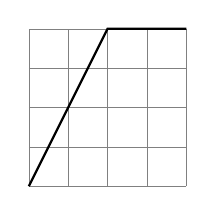
\begin{tikzpicture}
      \draw[step=0.5cm,gray,very thin] (0,0) grid (2,2);
      \draw[thick] (0,0) -- (1,2) -- (2,2);
    \end{tikzpicture}
    \quad
    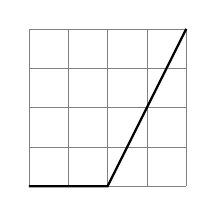
\begin{tikzpicture}
      \draw[step=0.5cm,gray,very thin] (0,0) grid (2,2);
      \draw[thick] (0,0) -- (1,0) -- (2,2);
    \end{tikzpicture}
    \quad
    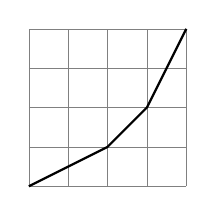
\begin{tikzpicture}
      \draw[step=0.5cm,gray,very thin] (0,0) grid (2,2);
      \draw[thick] (0,0) -- (1,0.5) -- (1.5,1) -- (2,2);
    \end{tikzpicture}
    \caption{Graphs of the functions $\phi_1$, $\phi_2$, and $\phi_3$ respectively.}
    \label{graph-reparametrisation}
  \end{figure}
  
  For (iii) we give a homotopy explicitly. Let us show that $\gamma \star \gamma^\inv \sim_p e_x$. For $t \in [0,1]$, define a path $\gamma_t : [0,1] \to X$ by $\gamma(s) = \gamma(ts)$, and define $G : [0,1] \times [0,1] \to X$ by
  \[
    G(s,t) = (\gamma_t \star \gamma_t^\inv)(s).
  \]
  That $G$ is continuous follows once again from an argument using Remark~\ref{pasting-closed}, and we see that $G$ is a homotopy from $e_x$ to $\gamma \star \gamma^\inv$ since
  \begin{align*}
    G(s,0) &= (\gamma_0 \star \gamma_0^\inv)(s) = \gamma(0) = x = e_x(s),\\
    G(s,1) &= (\gamma_1 \star \gamma_1^\inv)(s) = (\gamma \star \gamma^\inv)(s),\\
    G(0,t) &= \gamma_t(0) = \gamma(0) = x,\\
    G(1,t) &= \gamma_t^\inv(1) = \gamma(0) = x,
  \end{align*}
  for every $s$ and $t$. That $\gamma^\inv \star \gamma \sim_p e_y$ follows by an analogous argument.
\end{proof}


\subsection{The fundamental group}
The idea in this section will be to use the operation $\star$ on path homotopy classes to associate an algebraic structure to any pair $(X,x)$ for $X$ a topological space and $x \in X$. Moreover, when $X$ is path-connected, this structure will form a powerful topological invariant.

If $\gamma$ is a path from $x$ to $x$, we say that $\gamma$ is a \word{loop}{{\"o}gla} based at $x$.
\begin{defn}
  Let $X$ be a topological space, and let $x \in X$. Then the \word{fundamental group}{fundamentalgrupp} $\pi_1(X,x)$ is the set of all path homotopy classes of loops based at $x$. 
\end{defn}
\trans{fundamental group}{fundamentalgrupp}
To make sense of the terminology, let us recall a few basic notions from abstract algebra.
\begin{defn}
  A \word{group}{grupp} is a set $G$ with an operation $G \times G \to G$, denoted $(g,h) \mapsto g \cdot h$, an element $e \in G$ called a unit, and a bijection $G \to G$ denoted $x \mapsto x^{-1}$ called the inverse, so that
  \begin{itemize}
    \item $g \cdot (h \cdot k) = (g \cdot h) \cdot k$ for all $g,h,k \in G$,
    \item $e \cdot g = g = g \cdot e$ for all $g \in G$, and
    \item $g \cdot g^{-1} = g^{-1} \cdot g = e$ for all $g \in G$.
  \end{itemize}
  If $G$ and $H$ are groups, then a map $\phi : G \to H$ is called a \word{homomorphism}{homomorfi} if $\phi(g\cdot h) = \phi(g)\cdot\phi(h)$ for all $g,h \in G$. A bijective group homomorphism is called an \word{isomorphism}{isomorfi}.
\end{defn}
\trans{group}{grupp}
\trans{homomorphism}{homomorfi}
\trans{isomorphism}{isomorfi}
\begin{example}
  The one-point set $\{e\}$ is a group under the operation $(e,e) \mapsto e$. This group is called the \emph{trivial group}\index{trivial group}.
\end{example}
\begin{example}
  The integers form a group under the operation $(g,h) \mapsto g+h$. The unit is $0 \in \bbZ$, and if $n \in \bbZ$, then the inverse of $n$ is $-n$.
\end{example}
\begin{example}
  The set $\bbR \setminus \{0\}$ is a group with operation $(g,h) \mapsto gh$. The unit is $1$, and the inverse of $x \in \bbR \setminus \{0\}$ is $1/x$.
\end{example}
\begin{example}
  The set $\GL(n,\bbR)$ of invertible $(n \times n)$-matrices with entries in $\bbR$ is a group under matrix multiplication. The unit is the unit matrix.
\end{example}
\begin{prop}
  The fundamental group $\pi_1(X,x)$ is a group under the operation $\star$ on homotopy classes of loops for any topological space $X$ and any $x \in X$.
\end{prop}
\begin{proof}
  This follows immediately from Theorem~\ref{concatenation-homotopy}.
\end{proof} 

\begin{example}
  \label{fundemental-group-euclidean}
  In Example~\ref{euclidean-path-homotopy} we saw that any two given paths in $\bbR^n$ between the same points were homotopic. This in particular implies that any loop based at a point $x \in \bbR^n$ is null-homotopic; that is, homotopic to $e_x$. In other words,
  \[
    \pi_1(\bbR^n, x) = \{[e_x]\},
  \]
  the trivial group, for all $x \in \bbR^n$.
\end{example}
As the next thing, let us see how $\pi_1(X,x)$ depends on $x$.
\begin{thm}
  \label{fundamental-group-independent-of-basepoint}
  Let $X$ be a topological space, and let $\alpha$ be a path from $x$ to $y$ in $X$. Define a map $\hat{\alpha} : \pi_1(X,x) \to \pi_1(X,y)$ by
  \[
    \hat{\alpha}([\gamma]) = [\alpha^\inv] \star [\gamma] \star [\alpha].
  \]
  Then $\hat{\alpha}$ is well-defined and an isomorphism.
\end{thm}
\begin{proof}
  That $\hat{\alpha}$ is well-defined means that $\hat{\alpha}([\gamma]) = \hat{\alpha}([\gamma'])$ whenever $[\gamma] = [\gamma']$, i.e. $\gamma \sim_p \gamma'$. And indeed, if $F: [0,1] \times [0,1] \to X$ is a path homotopy from $\gamma$ to $\gamma'$, then $G : [0,1] \times [0,1] \to X$, defined by
  \[
    G(s,t) = (\alpha^\inv \star F(\cdot,t) \star \alpha)(s)
  \]
  is a path homotopy from $\alpha^\inv \star \gamma \star \alpha$ to $\alpha^\inv \star \gamma' \star \alpha$, so $\hat{\alpha}$ is well-defined.

  To see that $\hat{\alpha}$ is an homomorphism, notice that for any $[\gamma], [\gamma'] \in \pi_1(X,x)$, we have
  \begin{align*}
    \hat{\alpha}([\gamma]) \star \hat{\alpha}([\gamma']) &= [\alpha^\inv] \star [\gamma] \star [\alpha] \star [\alpha^\inv] \star [\gamma'] \star [\alpha] \\
      &= [\alpha^\inv] \star ([\gamma] \star [\gamma']) \star [\alpha] = \hat{\alpha}([\gamma] \star [\gamma']).
  \end{align*}
  To see that $\hat{\alpha}$ is a bijection, notice that $\widehat{\alpha^\inv} \circ \hat{\alpha}$ is the identity on $\pi_1(X,x)$ since for any $[\gamma] \in \pi_1(X,x)$, we have
  \[
    (\widehat{\alpha^\inv} \circ \hat{\alpha})[\gamma] = \widehat{\alpha^\inv}([\alpha^\inv] \star [\gamma] \star [\alpha]) = [\alpha] \star [\alpha^\inv] \star [\gamma] \star [\alpha] \star [\alpha^\inv] = [\gamma],
  \]
  and $\hat{\alpha} \circ \widehat{\alpha^\inv}$ is the identity on $\pi_1(X,y)$ by the same reasoning, so $\hat{\alpha}$ is a bijection and thus a group isomorphism.
\end{proof}
\begin{cor}
  If $X$ is a path-connected topological space, then $\pi_1(X,x)$ is independent of $x \in X$ up to isomorphism.
\end{cor}
Because of this result, one often writes $\pi_1(X) = \pi_1(X,x)$ for any $x \in X$ when $X$ is path-connected. It is then understood that the equality is really up to isomorphism.
\begin{defn}
  A topological space $X$ is called \word{simply-connected}{enkelt sammanh{\"a}ngande} if it is path-connected and $\pi_1(X)$ consists of a single element.
\end{defn}
\begin{example}
  By Example~\ref{fundemental-group-euclidean}, $\bbR^n$ is simply-connected.
\end{example}

The next result says that for path-connected spaces, $\pi_1$ is a topological invariant. Even when the spaces in question are not path-connected, one obtains a topological invariant by considering the collection of groups $\pi_1(X,x_i)$ up to isomorphism, where each of the $x_i$ belongs to a different path-component of $X$.

As preparation, suppose that $f : X \to Y$ is a continuous map, and let $x \in X$. Define a map
\[
  f_* : \pi_1(X,x) \to \pi_1(Y,f(x))
\]
by
\[
  f_*([\gamma]) = [f \circ \gamma].
\]

\begin{thm}
  Let $f : X \to Y$ and $g : Y \to Z$ be continuous maps, and let $x \in X$. Then
  \begin{itemize}
    \item[(i)] $f_*: \pi_1(X,x) \to \pi_1(Y,f(x))$ is a well-defined homomorphism,
    \item[(ii)] $(g \circ f)_* = g_* \circ f_*$, and if $\id : X \to X$ denotes the identity, then $\id_* : \pi_1(X,x) \to \pi_1(X,x)$ is the identity on $\pi_1(X,x)$.
    \item[(iii)] Finally, if $f$ is a homeomorphism, then $f_*$ is an isomorphism.
  \end{itemize}
\end{thm}
\begin{proof}
  That $f_*$ is well-defined means that $f \circ \gamma \sim_p f \circ \gamma'$ whenever $\gamma \sim_p \gamma'$. This is the case since if $F$ is a homotopy from $\gamma$ to $\gamma'$, then $f \circ F$ is a homotopy from $f \circ \gamma$ to $f \circ \gamma'$.
  
  To see that $f_*$ is a homomorphism, let $\gamma, \gamma' \in \pi_1(X,x)$. We first notice that by definition of concatenation, we have
  \[
    f \circ ( \gamma \star \gamma') = (f \circ \gamma) \star (f \circ \gamma'),
  \]
  from which it follows that
  \begin{align*}
    f_*([\gamma] \star [\gamma']) &= f_*([\gamma \star \gamma']) = [f \circ (\gamma \star \gamma')] = [(f \circ \gamma) \star (f \circ \gamma')] \\
      &= [ f \circ \gamma] \star [f \circ \gamma'] = f_*([\gamma]) \star f_*([\gamma']),
  \end{align*}
  so $f_*$ is a homomorphism, which shows (i).
  
  Similarly,
  \[
    (g_* \circ f_*)([\gamma]) = g_* ( [f \circ \gamma]) = [g \circ f \circ \gamma] = (g \circ f)_*([\gamma]),
  \]
  which shows the first part of (ii). The last part of (ii) is obvious.
  
  Finally, (iii) follows from (ii) as it follows that $(f^{-1})_*$ satisfies that both $f_* \circ (f^{-1})_*$ and $(f^{-1})_* \circ f_*$ are the identity homomorphisms. Thus $f_*$ is a bijection and therefore an isomorphism.
\end{proof} 

If $G$ and $H$ are two groups, then their Cartesian product $G \times H$ is a group with the group operation
\[
  (g,h) \cdot (g',h') = (g\cdot g', h \cdot h').
\]
\begin{prop}
  \label{product-fundamental-group}
  Let $X$ and $Y$ be topological spaces, and let $x \in X$, $y \in Y$. Then $\pi_1(X \times Y,(x,y))$ is isomorphic to $\pi_1(X,x) \times \pi_1(Y,y)$.
\end{prop}
\begin{proof}
  Exercise~\ref{product-fundamental-group-exercise}.
\end{proof}

\subsection{Covering spaces and fundamental groups of spheres}
The main result of this section is a calculation of $\pi_1(S^n)$ for all $n \geq 1$.
\begin{thm}
  \label{fundamental-group-of-spheres}
  We have $\pi_1(S^1) = \bbZ$, but $S^n$ is simply-connected for $n \geq 2$.
\end{thm}

To prove the case $n = 1$, it will be convenient to have at our disposal some basic results about covering spaces. Before going into any detail about these, let us consider the ``easy'' part of the claim.
\begin{proof}[Proof of Theorem~\ref{fundamental-group-of-spheres} for $n \geq 2$]
  Let $\gamma$ be a loop in $S^n$, based at some point $\gamma(0)$, and let us show that $\gamma$ is null-homotopic. If there is a point $p$ not in the image of $\gamma$, we can view $\gamma$ as a loop in $S^n \setminus \{p\}$, which is homeomorphic to $\bbR^n$ by Remark~\ref{south-pole-removed}. Since $\bbR^n$ is simply-connected, this tells us that $\gamma$ is null-homotopic as a loop in $S^n \setminus \{ p \}$ through some homotopy $[0,1] \times [0,1] \to S^n \setminus \{p\}$. By composition with the inclusion, this gives us a homotopy $[0,1] \times [0,1] \to S^n$, so $\gamma$ is also null-homotopic as a loop in $S^n$.
  
  This shows the claim in the case where $\gamma([0,1]) \not= S^n$, and let $p$ be a point in $S^n$ distinct from $\gamma(0)$. We will show how to make a path homotopy from $\gamma$ so some other loop, denoted $\gamma_k$ below, whose image does not contain $p$. This other loop will then be null-homotopic by the first part of the proof, so $\gamma$ will be as well.
  
  Let $U$ be any neighbourhood of $p$ which does not contain $\gamma(0)$. After possibly having to pass to a smaller neighbourhood we can assume that $U$ is homeomorphic to an open ball in $\bbR^n$. Now $\gamma^{-1}(U) \subset (0,1) \subset [0,1]$ is an open set and therefore a union of open disjoint intervals $\{(a_i,b_i)\}_{i \in I}$. Since $\{p\}$ is closed in $S^n$, $\gamma^{-1}(\{p\})$ is closed in $[0,1]$, and since $[0,1]$ is compact, so is $\gamma^{-1}(\{p\})$. Since $\{(a_i,b_i)\}_{i \in I}$ is an open cover of $\gamma^{-1}(\{p\})$ this compactness implies that we can find finitely many intervals $(a_1,b_1), \dots, (a_k,b_k)$ that cover $\gamma^{-1}(\{p\})$. We will now cook up the desired homotopy for each of these finitely many intervals.
  
  Since $(a_1,b_1) \subset \gamma^{-1}(U)$ with $a_1,b_1 \notin \gamma^{-1}(U)$, we get that $\gamma([a_1,b_1]) \subset \bar{U}$ and $\gamma(a_1),\gamma(b_1) \in \dd U$. Now take any path $\widetilde{\gamma_1}$ in $\bar{U}$ from $\gamma(a_1)$ to $\gamma(b_1)$ which does not go through $p$. Since $U$ was assumed to be homeomorphic to a ball, $\gamma|_{[a_1,b_1]}$ is path homotopic to $\widetilde{\gamma_1}$ (ignoring the minor detail that the paths in question have to be defined on $[0,1]$) and this path homotopy extends to a path homotopy from $\gamma$ to some loop $\gamma_1$ with the property that $p \notin \gamma_1([a_1,b_1])$ and so that $\gamma_1$ agrees with $\gamma$ on the complement of $[a_1,b_1]$ in $[0,1]$. We now iterate this procedure to obtain for each $j = 1, \dots, k$ a loop $\gamma_j$ so that $\gamma \sim_p \gamma_j$ and $p \notin \gamma_j([a_1,b_1] \cup \dots \cup [a_j,b_j])$. Then $p \notin \gamma_k([0,1])$ and $\gamma \sim \gamma_k$, so we are done.
\end{proof}

Before moving on to the case $n = 1$, let us notice the following non-trivial corollary of the theorem.
\begin{cor}
  We have $S^n \simeq T^m$ if and only if $n = m = 1$.
\end{cor}
\begin{proof}
  By Proposition~\ref{product-fundamental-group} and Theorem~\ref{fundamental-group-of-spheres}, $\pi_1(T^m) = \pi_1(S^1 \times \cdots \times S^1)$ is the product of $m$ copies of $\bbZ$. Since $\bbZ^m$ is not isomorphic to $\bbZ$ if $m > 1$, $\pi_1(T^m)$ can only be isomorphic to $\pi_1(S^n)$ if $n = m = 1$.
\end{proof}
\begin{wrapfigure}{R}{0.3\textwidth}
  \centering
  \begin{overpic}[width=0.28\textwidth]{images/covering}
    \put(37,60){$E$}
    \put(37,13){$B$}
    \put(24,33){$p$}
    \put(18,17){$U$}
    \put(13,91){$p^{-1}(U)$}
  \end{overpic}
  \caption{A covering map $p : E \to B$.}
  \label{covering-figure}
\end{wrapfigure}
% \trans{covering space}{?}
% \trans{covering map}{?}
\begin{defn}
  Let $B$ be a topological space. A \wordnotrans{covering space}{?} of $B$ is a topological space $E$ and a continuous surjective map $p : E \to B$, called a \wordnotrans{covering map}{?}, so that each point $b \in B$ has an open neighbourhood $U$ with the property that $p^{-1}(U)$ is a disjoint union of open sets in $E$, each of which is mapped homeomorphically to $U$ by $p$. See Figure~\ref{covering-figure}.
\end{defn}

\begin{example}
  \label{covering-of-circle}
  The real line $\bbR$ is a covering space of $S^1$ with covering map $p : \bbR \to S^1$ given by $p(x) = (\cos(2\pi x), \sin(2\pi x))$.
\end{example}

\begin{defn}
  Let $p : E \to B$ be a covering map, and let $f : X \to B$ be a continuous map. A map $\tilde{f} : X \to E$ is called a \word{lifting}{l{\"o}ft} of $f$ if $f = p \circ \tilde{f}$.
\end{defn}
\trans{lifting}{l{\"o}ft}

The two following lemmas will be proven in Section~\ref{proofs-lifting-lemmas} below.
\begin{lem}[Path lifting lemma]
  \label{path-lifting-lemma}
  \index{path lifting lemma}Let $p : E \to B$ be a covering map, let $b \in B$, and let $e \in E$ with $p(e) = b$. Then any path $\gamma : [0,1] \to B$ with $\gamma(0) = b$ has a unique lifting $\tilde{\gamma} : [0,1] \to E$ so that $\tilde{\gamma}(0) = e$.
\end{lem}

\begin{lem}[Homotopy lifting lemma]
  \label{homotopy-lifting-lemma}
  \index{homotopy lifting lemma}Let $p : E \to B$ be a covering map, and let $p(e) = b$ as above. Let $F : [0,1] \times [0,1] \to B$ be a homotopy with $F(0,0) = b$. Then there is a a unique lifting $\tilde{F} : [0,1] \times [0,1] \to E$ so that $\tilde{F}(0,0) = e$. If $F$ is a path homotopy then so is $\tilde{F}$.
\end{lem}

Now as above, let $p : E \to B$ be a covering map, let $b \in B$, and choose $e \in E$ with $p(e) = b$. Let $[\gamma] \in \pi_1(B,b)$ be a homotopy class of a path $\gamma$, and let $\tilde{\gamma}$ be the unique lifting from Lemma~\ref{path-lifting-lemma}, with $\tilde{\gamma}(0) = e$. Define a map, called the \word{lifting correspondence}{?},
\[
  \phi_e : \pi_1(B,b) \to p^{-1}(\{b\})
\]
by $\phi_e([\gamma]) = \tilde{\gamma}(1)$. To see that this is well-defined, assume that $\gamma \sim_p \gamma'$, and let $F$ denote a path homotopy from $\gamma$ to $\gamma'$. Then the unique lifting $\tilde{F}$ from Lemma~\ref{homotopy-lifting-lemma} is a path homotopy from $\tilde{\gamma}$ to $\widetilde{\gamma'}$, and in particular $\tilde{\gamma}(1) = \widetilde{\gamma'}(1)$.

\begin{prop}
  \label{lifting-correspondence-props}
  Let $p : E \to B$, $p(e) = b$, be as above. If $E$ is path-connected then $\phi_e$ is surjective. If $E$ is simply-connected, then $\phi_e$ is bijective.
\end{prop}
\begin{proof}
  Assume first that $E$ is path-connected and let $q \in p^{-1}(\{b\})$. Choose any path $\tilde{\gamma}$ from $e$ to $q$, and let $\gamma = p \circ \tilde{\gamma}$. Then $\tilde{\gamma}$ is a lift of $\gamma$ by construction, and $\phi_e([\gamma]) = q$, so $\phi_e$ is surjective.
  
  Assume now that $E$ is simply-connected, suppose that $\phi_e([\gamma]) = \phi_e([\gamma'])$ for two elements $[\gamma], [\gamma'] \in \pi_1(B,b)$, and let us show that $[\gamma] = [\gamma']$. Let $\tilde{\gamma}$ and $\widetilde{\gamma'}$ denote the corresponding lifts, so that $\tilde{\gamma}(1) = \tilde{\gamma'}(1)$ by assumption. Then $\tilde{\gamma} \star \widetilde{\gamma'}^\inv$ is a loop based at $e$ and thus path homotopic to the constant map since $E$ is simply-connected. This implies that
  \[
    [\tilde{\gamma}] = [\tilde{\gamma}] \star [\widetilde{\gamma'}^\inv] \star [\widetilde{\gamma'}] = [\tilde{\gamma} \star \widetilde{\gamma'}^\inv] \star [\widetilde{\gamma'}] = [\widetilde{\gamma'}],
  \]
  so there is a path homotopy $\tilde{F}$ from $\tilde{\gamma}$ to $\widetilde{\gamma'}$. Then $p \circ \tilde{F}$ is a path homotopy from $p \circ \tilde{\gamma} = \gamma$ to $p \circ \widetilde{\gamma'} = \gamma'$, or in other words, $[\gamma] = [\gamma']$.
\end{proof}

We are now in a position to prove our main result.
\begin{proof}[Proof of Theorem~\ref{fundamental-group-of-spheres} for $n = 1$]
  Let $p : \bbR \to S^1$ be the covering map from Example~\ref{covering-of-circle}, let $b = (1,0) \in S^1$, and let $e = 0$. In this case, since $p^{-1}(\{b\}) = \bbZ$, and since $\bbR$ is simply-connected, Proposition~\ref{lifting-correspondence-props} implies that $\phi_e : \pi_1(S^1,b) \to \bbZ$ is bijective, and we claim that it is a homomorphism.
  
  Let $m \in \bbZ$, and let $\gamma_m : [0,1] \to \bbZ$ be the loop given by
  \[
    \gamma_m(t) = (\cos(2\pi mt), \sin(2\pi mt)).
  \]
  This loop lifts to $\widetilde{\gamma_m} : [0,1] \to \bbR$ given by $\widetilde{\gamma_m}(t) = mt$. This tells us that $\phi_e([\gamma_m]) = m$. Since $\phi_e$ was a projection, each loop $\gamma$ based at $b$ will belong to $[\gamma_m]$ for some $m \in \bbZ$, so to show that $\phi_e$ is a homomorphism, it suffices to show that
  \[
    \phi_e([\gamma_m \star \gamma_n]) = m + n = \phi_e([\gamma_m]) + \phi_e([\gamma_n]),
  \]
  for all $m , n \in \bbZ$. Let $\widetilde{\gamma_n^m} = m + \widetilde{\gamma_n}$ be the lifting of $\gamma_n$ starting at $m$ and ending at $m+n$. Then $\widetilde{\gamma_m} \star \widetilde{\gamma_n^m}$ is a path from $0$ to $m+n$ and $p \circ (\widetilde{\gamma_m} \star \widetilde{\gamma_n^m}) = \gamma_m \star \gamma_n$, so by definition of $\phi_e$, this tells us that $\phi_e([\gamma_m \star \gamma_n]) = m+n$.
\end{proof}

Up until this point, it is not clear how useful $\pi_1$ actually is as an invariant: indeed, most of the calculations of fundamental groups that we have done turned out to yield trivial groups, and, for instance, we can not use the fundamental group to tell apart the spaces $\bbR^n$ and $S^n$ for $n \geq 2$, even though one can show by elementary means that these spaces are non-homeomorphic.

Restricting to the class of manifolds considered in Section~\ref{manifolds} one can say quite a bit more. It is not too difficult to prove, for instance, that if a $2$-manifold is compact and simply-connected, then it is homeomorphic to $S^2$. That is, the fundamental group can detect $S^2$ among all compact $2$-manifolds. The same statement holds true for $3$-manifolds, although it is currently significantly harder to prove.
\begin{thm}[The Poincar{\'e} conjecture]
  \index{Poincar{\'e} conjecture}If $X$ is a simply-connected compact $3$-manifold, then $X \simeq S^3$.
\end{thm}
Conjectured by Henri Poincar{\'e} in 1904, and first proven by Grigori Perelman in 2003, at the time of writing this is the only solved out of the seven so-called Millennium Prize Problems\footnote{See \url{https://en.wikipedia.org/wiki/Millennium_Prize_Problems}.}.

\subsection{Proofs of lifting lemmas}
\label{proofs-lifting-lemmas}
We now turn to the proofs of Lemmas~\ref{path-lifting-lemma} and \ref{homotopy-lifting-lemma} where we will need a technical result on subdivisions of $[0,1]$ and $[0,1] \times [0,1]$. We word it here for general compact metric spaces.

Let $(X,d)$ be a metric space, and let $A$ be a non-empty subset. Then for every $x \in X$, we define the distance from $x$ to $A$ by
\[
  d(x,A) = \inf \{ d(x,a) \mid a \in A \}.
\]
It is easy to see that for fixed $A$, the function $x \mapsto d(x,A)$ is continuous. If moreover $A$ is bounded in the sense that the set $\{d(a_1,a_2) \mid a_1,a_2 \in A\} \subset \bbR$ is bounded, we define the \word{diameter}{diameter} of $A$ to be
\[
  \diam(A) = \sup \{d(a_1,a_2) \mid a_1,a_2 \in A \} \in \bbR.
\]
\begin{lem}[Lebesgue's number lemma]
  \label{lebesgue-number-lemma}
  \index{Lebesgue's number lemma}Let $\calU$ be an open cover of a compact metric space $(X,d)$. Then there is a $\delta > 0$, called a \index{Lebesgue number}\emph{Lebesgue number}, so that for every subset $A$ of diameter less than $\delta$, there is a $U \in \calU$ with $A \subset U$.
\end{lem}
\begin{proof}
  First of all, if $X \in \calU$, we are done since any $\delta > 0$ does the job, so assume that $X \notin \calU$.

  Now use the compactness of $X$ to take an finite subcover $\{U_1,\dots,U_n\} \subset \calU$. Let $C_i = X \setminus U_i \not= \emptyset$ for $i = 1, \dots, n$, and define a function $f : X \to \bbR$ by
  \[
    f(x) = \frac{1}{n} \sum_{i=1}^n d(x,C_i).
  \]
  We claim that $f(x) > 0$ for all $x \in X$. To see this, let $x \in X$ and choose an $i$ so that $x \in U_i$. Since $U_i$ is open, we can find a $\eps > 0$ so that $B(x,\eps) \subset U_i$. Then $d(x,C_i) \geq \eps$, so $f(x) \geq \eps/n > 0$. Since $f$ is continuous, it follows from Corollary~\ref{sup-inf-compact-continuous} that $f(X)$ has a minimum $\delta > 0$, and we now claim that this number is our desired Lebesgue number.
  
  Let $A \subset X$ have diameter less than $\delta$, and let $a \in A$. Then $A \subset B_d(a,\delta)$, and by taking $m \in \{1,\dots,n\}$ so that $d(a,C_m)$ is maximal, we have
  \[
    \delta \leq f(a) \leq d(a,C_m),
  \]
  so $A \subset B_d(a,\delta) \subset X \setminus C_m = U_m$.
\end{proof}
We can now prove the two lemmas.% As will be clear, the two proofs are very similar, and indeed one could view both of them as following from a more general result on liftings of homotopies. To simplify the exposition, however, we prove the claims separately.
\begin{proof}[Proof of Lemma~\ref{path-lifting-lemma}]
  Choose an open cover $\calU$ of $B$ by sets $U \in \calU$ with the property that $p^{-1}(U)$ is a disjoint union of open sets in $E$, each of which is mapped homeomorphically to $U$ by $p$.
  
  Now $\{\gamma^{-1}(U) \mid U \in \calU\}$ is an open cover of the compact set $[0,1]$. By Lemma~\ref{lebesgue-number-lemma}, there is a subdivision $0 = s_0 < s_1 < \dots < s_n = 1$ of $[0,1]$ so that for every $i = 1, \dots, k$, we have $[s_{i-1},s_i] \subset \gamma^{-1}(U)$ for some $U \in \calU$. That is, $\gamma([s_{i-1},s_i]) \subset U$. We will now construct the lifting $\tilde{\gamma}$ on each of these smaller intervals through a finite induction.
  
  Let $\tilde{\gamma}(0) = e$ and assume that the lifting $\tilde{\gamma}$ has been defined on $[0,s_i]$. We then define $\tilde{\gamma}$ on $[s_i,s_{i+1}]$ as follows: let $V \in \calU$ be the open set so that $\gamma([s_i,s_{i+1}]) \subset U$. Then $\tilde{\gamma}(s_i) \in p^{-1}(U)$, so we can choose $V \subset E$ so that $p|_V : V \to U$ is a homeomorphism and $\tilde{\gamma}(s_i) \in V$. Now, for any $s \in [s_i,s_{i+1}]$, we can define
  \[
    \tilde{\gamma}(s) = (p|_V)^{-1}(\gamma(s)).
  \]
  Then $\tilde{\gamma}$ is continuous on $[s_i,s_{i+1}]$, agrees with $\tilde{\gamma}$ on the set $\{s_i\}$, and so defines a function $\tilde{\gamma} : [0,s_{i+1}] \to E$ which is continuous by the pasting lemma, Remark~\ref{pasting-closed}. Moreover, $\tilde{\gamma}$ is constructed to satisfy $\gamma = p \circ \tilde{\gamma}$ where it is defined, so repeating this procedure $n$ times we obtain our desired lift.
  
  It remains to prove that $\tilde{\gamma}$ is unique. Suppose that $\tilde{\gamma}'$ is another lifting of $\gamma$ with $\tilde{\gamma}'(0) = e$, and suppose that $\tilde{\gamma} = \tilde{\gamma}'$ on $[0,s_i]$ (which we know is true for $i=0$). We then claim that the lifts agree on $[0,s_{i+1}]$ as well, and therefore $\tilde{\gamma} = \tilde{\gamma}'$ on all of $[0,1]$, so let $s \in [s_i,s_{i+1}]$, and let $V$ be as above so that $\tilde{\gamma}(s_i), \tilde{\gamma}'(s_i) \in V$.
  
  Since $[s_i,s_{i+1}]$ is connected, so is the set $\tilde{\gamma}'([s_i,s_{i+1}])$ by Theorem~\ref{images-of-connected}, and therefore it must be contained in a single connected component by Proposition~\ref{props-of-conn-components}. Now, since the open sets making up $p^{-1}(U)$ are disjoint, this implies that $\tilde{\gamma}'([s_i,s_{i+1}]) \subset V$, so in particular $\tilde{\gamma}'(s) \in V$. Now, since $p|_V : V \to U$ is bijective, there is only one point in $V$ that is mapped to $\gamma(s)$ under $p$, namely $(p|_V)^{-1}(\gamma(s))$, so since $\tilde{\gamma}'$ is a lifting of $\gamma$, it follows that
  \[
    \tilde{\gamma}'(s) = (p|_V)^{-1}(\gamma(s)) = \tilde{\gamma}(s).
  \]
\end{proof}

\begin{proof}[Proof of Lemma~\ref{homotopy-lifting-lemma}]
  \begin{figure}
    \centering
    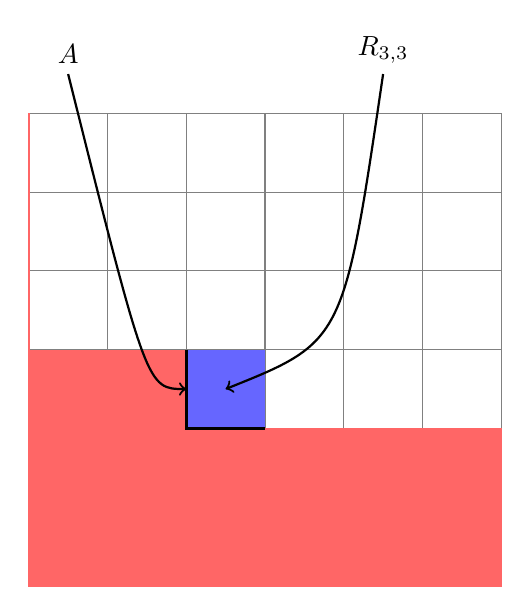
\begin{tikzpicture}
      \draw[step=1cm,gray] (0,0) grid (6,6);
      \fill[red!60!white] (0,0) rectangle (2,3);
      \fill[red!60!white] (0,0) rectangle (6,2);
      \fill[blue!60!white] (2,2) rectangle (3,3);
      \draw[red!60!white,thick] (0,6) -- (0,0) -- (6,0) -- (6,2);% -- (3,2);
      %\draw[red!60!white,thick] (0,3) -- (2,3);
      %\draw[blue!60!white,thick] (3,2) -- (3,3) -- (2,3);
      \draw[very thick] (2,3) -- (2,2) -- (3,2);
      \draw[thick,<-] (2.5,2.5) .. controls (4,3.1) .. (4.5,6.5) node[anchor=south]{$R_{3,3}$};
      \draw[thick,<-] (2,2.5) .. controls (1.5,2.5) .. (0.5,6.5) node[anchor=south]{$A$};
    \end{tikzpicture}
    \caption{The sets involved in the proof of Lemma~\ref{homotopy-lifting-lemma}. The red part indicates where $\tilde{F}$ has been defined, and the blue part where we are in the process of defining $\tilde{F}$.}
    \label{homotopy-lifting-figure}
  \end{figure}
  As in the proof above, we will define a lift $\tilde{F}$ in a step-by-step fashion, so let $\calU$ denote an open cover $B$ as above. Begin by letting $\tilde{F}(0,0) = e$, and use Lemma~\ref{path-lifting-lemma} to uniquely define $\tilde{F}$ on $[0,1] \times \{0\}$ and $\{0\} \times [0,1]$, lifting $F$ on these subsets.
  
  As above, we can now consider $\{F^{-1}(U) \mid U \in \calU\}$ and conclude by Lemma~\ref{lebesgue-number-lemma} that there exist subdivisions $0 = s_0 < s_1 < \dots < s_m = 1$ and $0 = t_0 < t_1 < \dots < t_n = 1$ so that for each rectangle
  \[
    R_{i,j} = [s_{i-1},s_i] \times [t_{j-1},t_j] \subset [0,1] \times [0,1]
  \]
  there is a $U \in \calU$ with $F(R_{i,j}) \subset U$. We now define $\tilde{F}$ on the rectangles $R_{i,j}$ in the order
  \[
    R_{1,1}, R_{2,1}, \dots, R_{m,1}, R_{1,2}, R_{2,2}, \dots, R_{m,2}, \dots, R_{1,n}, R_{2,n}, \dots, R_{m,n}.
  \]
  Assume that the lifting $\tilde{F}$ has been defined on all rectangles up to a certain point, and let us define $\tilde{F}$ on the next rectangle $R_{i,j}$. In particular, $\tilde{F}$ has been defined on $A$: the union of the left and bottom edge of $R_{i,j}$, which is a connected set (see Figure~\ref{homotopy-lifting-figure}). By the exact same logic as in the previous proof, this implies $\tilde{F}(A) \subset V$, where $V \subset E$ is so that $p|_V : V \to U$ is a homeomorphism and $F(R_{i,j}) \subset U$. This means that we can extend $\tilde{F}$ to $R_{i,j}$ by letting
  \[
    \tilde{F}(x) = (p|_V)^{-1}(F(x)).
  \]
  Proceeding like this for all rectangles, we define $\tilde{F}$ on all of $[0,1] \times [0,1]$. Then $\tilde{F}$ is continuous by the pasting lemma and a lifting of $F$ by construction. That $\tilde{F}$ is the unique lifting with $\tilde{F}(0,0) = e$ follows by the same logic as in the proof of Lemma~\ref{path-lifting-lemma} above.
  
  It remains to show that if $F$ is a path homotopy, then so is $\tilde{F}$. So, assume that $F([0,1] \times \{0\}) = \{b\}$. Then $\tilde{F}([0,1]\times\{0\}) \subset p^{-1}(\{b\})$. Now $[0,1] \times \{0\}$ is connected, so its image under $\tilde{F}$ is connected, and on the other hand, $p^{-1}(\{b\})$ is discrete so its connected components are points, which means that $\tilde{F}$ is constant on $[0,1] \times \{0\}$. Similarly, if $F$ is constant on $[0,1] \times \{1\}$, one uses connectedness to argue that $\tilde{F}$ is as well.
\end{proof}

\section{Manifolds}
\label{manifolds}
The concept of a manifold is central in all of differential geometry and mathematical physics; roughly, a manifold is a topological space which locally looks like $\bbR^n$. Another way of viewing it is that a manifold is something which is obtained by gluing together copies of $\bbR^n$. As such, its usefulness in for instance geometry comes from the fact that we can transfer everything we know about calculus on $\bbR^n$ to this much more general family of topological spaces, as long as one ensures that the gluing is sufficiently compatible with calculus. Now, we will not be discussing calculus here but rather take a look at manifolds from a purely topological point of view.

\subsection{Topological manifolds}
\begin{defn}
  An \emph{$n$-dimensional} \word{manifold}{m{\aa}ngfald} or simply an \emph{$n$-manifold} is a second countable Hausdorff space such that every point has a neighbourhood which is homeomorphic to $\bbR^n$.
\end{defn}
\trans{manifold}{m{\aa}ngfald}
Really what we have defined above is a \emph{topological manifold}\index{topological manifold}; since this is the only kind of manifold we will encounter, we will simply call them ``manifolds''.
\begin{example}
  Euclidean space $\bbR^n$ is a manifold since $\bbR^n$ itself is a neighbourhood of all of its points.
\end{example}
\begin{example}
  \label{spheres-are-manifolds}
  The $n$-sphere $S^n$ is a manifold. If $x \in S^n$ is a point different from the north pole $p = (0,\dots,0,1)$, then $S^n \setminus \{p\}$ is a neighbourhood of $x$ which is homeomorphic to $\bbR^n$ by Proposition~\ref{north-pole-removed}. If $x = p$, let $q$ denote the south pole. Then $S^n \setminus \{q\}$ is a neighbourhood of $x$ which is homeomorphic to $\bbR^n$ by Remark~\ref{south-pole-removed}.
\end{example}
\begin{lem}
  \label{products-of-manifolds-lemma}
  The product of an $n$-manifold and an $m$-manifold is an $(n+m)$-manifold.
\end{lem}
\begin{proof}
  Exercise~\ref{products-of-manifolds-exercise}.
\end{proof}
\begin{example}
  The $n$-torus $T^n$ is an $n$-manifold by Lemma~\ref{products-of-manifolds-lemma} and Example~\ref{spheres-are-manifolds}.
\end{example}
\begin{example}
  The genus $g$ surfaces $\Sigma_g$ from Example~\ref{surface-example} are $2$-manifolds.
\end{example}

\subsection{Embeddings of manifolds}
Notice that by definition, $S^n$ can be embedded in $\bbR^{n+1}$. Similarly, $T^n$ can be embedded in $\bbR^{2n}$, and Figures~\ref{genus-1-surface}-\ref{genus-3-surface} suggest that $\Sigma_g$ can be embedded in $\bbR^3$.

In this section we will see how to use Urysohn's lemma to show the following result.
\begin{thm}
  Any compact $n$-manifold can be embedded in $\bbR^N$ for some $N \in \bbN$.
\end{thm}
\begin{defn}
  Let $X$ be a topological space and $f : X \to \bbR$ a function. The \word{support}{?} of $f$ is the set
  \[
    \supp(f) = \bar{\{x \mid f(x) \not= 0\}}.
  \]
\end{defn}
\trans{support}{?}
\begin{defn}
  Let $X$ be a topological space, and let $\{U_1, \dots, U_n\}$ be an open cover of $X$. A family $\{\phi_1,\dots,\phi_n\}$ of continuous functions $\phi_i : X \to [0,1]$ is called a \word{partition of unity}{?} dominated by $\{U_i\}$ if
  \begin{itemize}
    \item $\supp(\phi_i) \subset U_i$ for $i = 1, \dots, n$, and
    \item $\sum_{i=1}^n \phi_i(x) = 1$ for all $x \in X$.
  \end{itemize}
\end{defn}
\trans{partition of unity}{?}
\begin{thm}
  Let $X$ be a $T_4$-space, and let $\{U_1, \dots, U_n\}$ be a finite open cover. Then there exists a partition of unity dominated by $\{U_1,\dots,U_n\}$.
\end{thm}
\begin{proof}
  We first show that we can find an open cover $\{V_1, \dots, V_n\}$ so that $\bar{V_i} \subset U_i$ for all $i$. Consider the set $A_1 = X \setminus (U_2 \cup \dots \cup U_n)$. This is clearly closed, and $A_1 \subset U_1$ since $\{U_i\}$ is a cover. Since $X$ is $T_4$, by Theorem~\ref{separation-squeeze-lemma} we obtain an open set $V_1$ so that $A_1 \subset V_1 \subset \bar{V_1} \subset U_1$, and in particular $\{V_1,U_2,\dots,U_n\}$ is still an open cover. We proceed now by finite induction: suppose that $\{V_1, \dots, V_{k-1},U_k,\dots,U_n\}$ covers $X$, and let
  \[
    A_k = X \setminus (V_1 \cup \dots \cup V_{k-1} \cup U_{k+1} \cup \dots \cup U_n).
  \]
  Then $A_k \subset U_k$, and we find as above an open set $V_k$ with $A_k \subset V_k \subset \bar{V_k} \subset U_k$ so that $\{V_1, \dots, V_k, U_{k+1}, \dots, U_n\}$.
  
  Now go through the same procedure again to obtain an open cover $\{W_1, \dots, W_n\}$ with $\bar{W_i} \subset V_i$ for all $i$. Applying Urysohn's lemma for each $i = 1, \dots, n$, we find continuous functions $\psi_i : X \to [0,1]$ so that $f(X \setminus V_i) = \{0\}$ and $f(\bar{W_i}) = \{1\}$. It follows that
  \[
    \supp(\psi_i) \subset \bar{V_i} \subset U_i.
  \]
  Since $\{W_i\}$ is a cover of $X$, it follows that $\psi(x) = \sum_{i=1}^n \psi_i(x) > 0$ for all $x$. Now define $\phi_i : X \to [0,1]$ by
  \[
    \phi_i(x) = \frac{\psi_i(x)}{\psi(x)}.
  \]
  We then have $\supp(\phi_i) = \supp(\psi_i) \subset U_i$, and for every $x \in X$, we have
  \[
    \sum_{i=1}^n \phi_i(x) = \frac{1}{\psi(x)} \sum_{i=1}^n \psi_i(x) = 1,
  \]
  so $\{\phi_i\}$ is a partition of unity dominated by $\{U_1,\dots,U_n\}$.
\end{proof}


\backmatter
\appendix
\section{Exercises}
The exercises are split into four sets, corresponding to the four exercise sessions held as part of the course. Many of the exercises are collected from previous iterations of the course, and these in turn may originate from \cite{Mun}. A few have been inspired by exercises in \cite{DM}.

\subsection{Set \#1}
\begin{enumerate}[label=1.\arabic*]
  \item Define a relation on $\bbR$ by
    \[
      C=\{(x,y) \mid x - y \in \bbZ \}.
    \]
    Show that $C$ is an equivalence relation and describe the set of equivalence classes of $C$.
  \item Describe all possible topologies on the set $X = \{a,b,c\}$.
  \item Let $X$ be a set, and let $\calT_1$ and $\calT_2$ be two different topologies on $X$. When is the identity map $\id : X \to X$ given by $\id(x) = x$ a continuous map from $(X,\calT_1)$ to $(X,\calT_2)$?
  \item
		Show that the subspace topology $\calT_Y$ is the smallest (meaning coarsest) topology on $Y\subset X$ for which the inclusion $\iota:Y \rightarrow X$ is a continuous map.
	
	\item \label{opens-in-opens} Let $Y\subset X$ be an open (closed) subset of a topological space $X$. Show that a set $U \subset Y$ is open (closed) in the subspace topology on $Y$ if and only if $U$ is open (closed) in $X$.
	
	\item \label{universal-inclusion} Prove Lemma~\ref{universal-inclusion-lemma}.
	
  \item \begin{itemize}
		\item[($a$)] Describe the open sets in the poset topology on $\{a,b,c,d\}$ defined by the relations $a\preceq b\preceq c$ and $a\preceq d$.
		\item[($b$)] Describe the open sets in the poset topology on $(\bbR,\leq)$.
	\end{itemize}
	
  \item The Euclidean space $\bbR^2$ can be identified with the Cartesian product $\bbR \times \bbR$. Use Lemma~\ref{compare-bases} to show that the standard topology on $\bbR^2$ equals the product topology on $\bbR \times \bbR$ (where each $\bbR$ has the standard topology).
  

  \item \label{metric-Hausdorff} Show that metric spaces are always Hausdorff.
  
  \item \label{subspace-Hausdorff} Show that if $X$ is Hausdorff, then so is any subset $Y\subset X$ with the subspace topology.
  
  \item \label{products-Hausdorff} Show that the product of two Hausdorff spaces is Hausdorff.
  
  \item Show that a topological space $X$ is Hausdorff if and only if the diagonal
  \[
    \Delta = \{(x,x) \in X \times X \mid x \in X \} \subset X \times X
  \]
  is closed in the product topology on $X \times X$.
  
  \item \label{metric-first-countable} Let $(X,d)$ be a metric space, and let
  \[
    \calB = \{ B_d(x,1/n) \mid x \in X, n \in \bbN \}.
  \]
  Show that $\calB$ is a basis for the metric topology on $X$.
  
  \item Let $(Y,\preceq)$ be a totally ordered set made into a topological space with the order topology.
  \begin{itemize}
    \item[($a$)] Show that for any two distinct points $x, y \in Y$ there are disjoint neighbourhoods, $U$ and $V$, of $x$ and $y$ respectively, so that $u < v$ for all $u \in U, v \in V$. Conclude that $Y$ is Hausdorff.
    \item[($b$)] Let $X$ be any topological space, and let $f,g:X\to Y$ be two continuous functions. Show that the set $\{x \mid f(x)\preceq g(x)\}$ is closed in $X$.
  \end{itemize}
  
  \item \label{product-metric}Let $(X_1,d_1)$ and $(X_2,d_2)$ be metric spaces. Define a metric on $X_1 \times X_2$ by
	\[
	  d((x_1,x_2),(y_1,y_2)) = \max(d_1(x_1,y_1),d_2(x_2,y_2)).
  \]
  Show that the metric topology on $X_1 \times X_2$ induced by $d$ is the product topology, where $X_1$ and $X_2$ have the metric topologies from $d_1$ and $d_2$ respectively.

  
  \item Let $X,Y,Z$ be topological spaces and consider a function $F:X\times Y\rightarrow Z$. We say that $F$ is \emph{continuous in each variable} if for each $y_0\in Y$ the function $h:X\rightarrow Z$ defined by $h(x)=F(x,y_0)$ is continuous, \emph{and} if for each $x_0\in X$ the function $g:Y\rightarrow Z$ defined by $g(y) = F(x_0,y)$ is continuous. Show that if $F$ is continuous, then $F$ is continuous in each variable.
  
  \item \begin{itemize}
		\item[($a$)] A poset topology is $T_0$. When is it $T_1$?
		\item[($b$)] If $X$ is a $T_0$-space with finitely many elements. Then we can define a relation
		\[x\preceq y \Leftrightarrow y\in \bigcap_{U\subset X\text{ open}, \,x\in U} U.\]
		Show that $\preceq$ is a partial order. What is the poset topology on $(X,\preceq)$?
	\end{itemize}
\end{enumerate}

\subsection{Set \#2}
\begin{enumerate}[label=2.\arabic*]
  \item Show that a topological space $X$ is connected if and only if the following condition holds: if $X = C \cup D$ where $C$ and $D$ are disjoint closed subsets of $X$, then either $C = \emptyset$ or $D = \emptyset$.
  \item Let $X = \{a,b,c\}$ with the topology $\{\emptyset,\{a,b\},\{c\},\{a,b,c\}\}$. Is $X$ connected? Path-connected?
  \item Consider the topology on $\bbR$ generated by the basis $\{(a,\infty) \mid a \in \bbR \}$, and let $x_0 \in \bbR$. \begin{itemize}
    \item[($a$)] What is $\{x_0\}'$, the set of limit points of $\{x_0\}$?
    \item[($b$)] What is the closure $\bar{\{x_0\}}$?
    \item[($c$)] Is $\bbR$ Hausdorff in this topology?
  \end{itemize}
  \item \label{connected-implies-interval} Show that the connected subsets of $\bbR$ are exactly the intervals.
  \item \label{origin-removed-connected} Show that $\bbR^n \setminus \{0\}$ is connected when $n \geq 2$.
  \item \label{invariance-of-dimension-exercise} Show that $\bbR^n \not\simeq \bbR$ when $n > 1$.
  \item Show that the concatenation $\gamma_1 \star \gamma_2$ is continuous by using Theorem~\ref{sequential-continuity} instead of the pasting lemma.
  \item Show that $S^n$ is path-connected for every $n > 0$.
  \item Let $p : X \to Y$ be a quotient map. Show that if $X$ is locally connected then so is $Y$.
  \item \label{locally-connected-open} Show that the connected components of a locally connected space are open.
  \item Let $\{A_n\}_{n \in \bbN}$ be a family of connected subspaces of a topological space $X$ so that $A_n \cap A_{n+1} \not= \emptyset$ for every $n \in \bbN$. Show that $\bigcup_{n \in \bbN} A_n$ is connected.
  \item A space is called \emph{totally disconnected} if its only connected subspaces are one-point sets. Show that if $X$ has the discrete topology, then $X$ is totally disconnected. Does the converse hold?
  \item Let $f : S^1 \to \bbR$ be continuous. Show that there is a point $x \in S^1$ so that $f(x) = f(-x)$.
  \item Let $f : [0,1] \to [0,1]$ be continuous. Show that $f$ has a fixed point, i.e. that there is a point $x \in [0,1]$ so that $f(x) = x$.
  \item \label{exercise-products-connected} Show Theorem~\ref{products-connected} in the case where $I$ is infinite. Inspiration can be found in \cite[Ex.~23.7]{Mun}.
\end{enumerate}

\subsection{Set \#3}
  \begin{enumerate}[label=3.\arabic*]
    \item \label{one-point-exercise}Let $X$ be a topological space.
    \begin{itemize}
      \item[(a)] Show that if $K_1, \dots, K_n$ are compact subspaces, then $K_1 \cup \dots \cup K_n$ is compact.
      \item[(b)] Suppose that $X$ is Hausdorff. Show that if $\{K_i\}_{i \in I}$ is a family of compact subspaces of $X$, then $\bigcap_{i \in I} K_i$ is compact.
      \item[(c)] Prove Proposition~\ref{one-point}.
    \end{itemize}
    \item \label{compact-hausdorff-are-normal-exercise} Show that compact Hausdorff spaces are normal.
    \item \label{local-compactness-in-hausdorff-exercise}Prove Theorem~\ref{local-compactness-in-hausdorff} (Hint: Use the one-point compactification.)
    \item \label{one-point-compactification-unique-exercise}Prove Proposition~\ref{one-point-compactification-unique}.
    \item Show that if $X$ is $T_3$ and $C \subset X$ a closed subset, then the quotient space $X/C$ is Hausdorff.
    \item \label{second-countable-exercise}Show that $\{B(x,r) \mid x \in \bbQ^n, r \in \bbQ_{> 0}\}$ is a basis for the standard topology on $\bbR^n$. Conclude that $\bbR^n$ is second-countable.
    \item Let $Y$ be a compact space, and let $X$ be any topological space.
      \begin{itemize}
      \item[(a)] Show the canonical projection map $\pi : X \times Y \to X$ is closed, i.e. that images of closed sets are closed.
      \item[(b)] Suppose moreover that $Y$ is Hausdorff, and let $f : X \to Y$ be a map. Show that $f$ is continuous if and only if its graph
        \[
          G_f = \{(x,f(x)) \mid x \in X\} \subset X \times Y
        \]
        is closed.
      \end{itemize}
    \item Let $(X,\preceq)$ be a totally ordered set with the order topology, and assume that all every closed interval $[a,b]$ is compact. Show that $X$ has the \emph{least-upper-bound property}\index{least-upper-bound property}; that is, show that every non-empty subset of $X$ which is bounded from above has a least upper bound in $X$.
    \item \label{baires-exercise} Let $X$ be a locally compact Hausdorff space, and let $U_1, U_2, U_3, \dots$ be open dense subsets of $X$. Show that $\bigcap_{n \in \bbN} U_n$ is dense; a result known as the Baire category theorem\index{Baire category theorem}. Hints:
      \begin{itemize}
        \item[(a)] Let $B_0$ be any non-empty open subset of $X$. Construct open sets $B_1, B_2, \dots$ so that
          \[
            \bar{B_n} \subset U_n \cap B_{n-1}
          \]
          for $n \geq 1$ and so that $\bar{B_n}$ is compact for all $n$.
        \item[(b)] Let $K_1, K_2, \dots$ be non-empty compact subsets of a topological space. Show that if we have inclusions $K_1 \supset K_2 \supset \cdots$, then
          \[
            \bigcap_{n \in \bbN} K_n \not= \emptyset.
          \]
          This result is known as Cantor's intersection theorem\index{Cantor's intersection theorem}.
      \end{itemize}
      What happens if we replace the countable family $\{U_n\}_{n \in \bbN}$ with an arbitrary family of open dense subsets?
    \item Let $X$ be a locally compact Hausdorff space, and let $\{F_n\}_{n \in \bbN}$ be a countable family of closed subsets of $X$. Show that if $\Int(F_m) = \emptyset$ for every $m \in \bbN$, then $\Int\left(\bigcup_{n \in \bbN} F_n\right) = \emptyset$. (Hint: use Exercise~\ref{baires-exercise}.)
%     \item Let $X$ be a sequentially compact topological space.
%       \begin{itemize}
%         \item[(a)] If $f : X \to Y$ is continuous, does it follow that $f(X)$ is sequentially compact?
%         \item[(b)] If $C \subset X$ is closed, does it follow that $C$ is sequentially compact?
%         \item[(c)] If $X$ is a subspace of a Hausdorff space $Z$, does it follow that $X$ is closed in $Z$?
%       \end{itemize}
%   \item Let $(X,d)$ be a metric space. A function $f : X \to X$ satisfying
%     \[
%       d(f(x),f(y)) = d(x,y)  
%     \]
%     for all $x, y \in X$ is called an \word{isometry}{isometri} of $X$. Show that if $f$ is an isometry, and $X$ is compact, then $f$ is a homeomorphism. Hint: if $a \in f(X)$, choose $\eps > 0$ so that $B_d(a,\eps) \cap f(X) = \emptyset$. Construct recursively a sequence $\{x_n\}$ so that $x_1 = a$, $x_{n+1} = f(x_n)$ and show that $d(x_m,x_n) \geq \eps$ for $n \not= m$.
%   \item Show that the one-point compactification of $\bbN \subset \bbR$ is homeomorphic to
%     \[
%       \{0 \} \cup \{1/n \mid n \in \bbN \} \subset \bbR.
%     \]
  \end{enumerate}
  
\subsection{Set \#4}
\begin{enumerate}[label=4.\arabic*]
  \item \label{products-of-manifolds-exercise} Prove Lemma~\ref{products-of-manifolds-lemma}.
  \item \label{invariance-of-dimension-manifolds} Use Theorem~\ref{invariance-of-dimension} to show that if $X$ is both an $n$-manifold and an $m$-manifold, then $m = n$.
\end{enumerate}

\printindex
\section{Dictionary}
\label{dictionary}
% Once more, this is taken from
%   https://tex.stackexchange.com/questions/19746/cunning-latex-tricks/19761#19761

\begin{longtable}{llll}
  \toprule[1pt]
  English & Swedish \\
  \midrule
  \@for\i:=\alist \do{\csname\i\endcsname}
  \vspace{-14pt}\\\bottomrule
\end{longtable}


\setlength\bibitemsep{0pt}
\bibliographystyle{is-alpha}
\bibliography{references}

\end{document}
